\chapter{ارزیابی و نتایج یادگیری}

در این فصل، نتایج حاصل از فرآیند یادگیری تقویتی در محیط سه‌جسمی ارائه و تحلیل شده است. هدف، بررسی عملکرد الگوریتم‌های استفاده‌شده و ارزیابی توانایی آن‌ها در دستیابی به اهداف تعیین‌شده می‌باشد. الگوریتم‌های یادگیری تقویتی مختلف شامل \lr{DDPG}، \lr{PPO}، \lr{SAC} و \lr{TD3} در دو حالت تک‌عاملی و چندعاملی مبتنی بر بازی مجموع‌صفر مورد بررسی قرار گرفته‌اند. این فصل به ارائه نتایج عملکردی این الگوریتم‌ها و مقایسه قابلیت‌های آن‌ها در شرایط مختلف می‌پردازد. در بخش \ref{sec:experimental_setup} تنظیمات آزمایشی و پارامترهای محیط شبیه‌سازی معرفی می‌شوند. بخش \ref{sec:trajectory_comparison} به مقایسه مسیرها و فرمان‌های پیشران الگوریتم‌های مختلف در حالت‌های تک‌عاملی و چندعاملی می‌پردازد. ارزیابی مقاومت الگوریتم‌ها در برابر شرایط مختلف اختلال در بخش \ref{sec:robustness_evaluation} بررسی می‌شود. در بخش \ref{sec:comprehensive_comparison} مقایسه جامع بین تمام الگوریتم‌ها ارائه می‌گردد. تحلیل پایداری و همگرایی الگوریتم‌ها در بخش \ref{sec:stability_analysis} مورد بررسی قرار می‌گیرد و در نهایت در بخش \ref{sec:benchmark_comparison} مقایسه با معیارهای مرجع انجام می‌شود.








\section{ارزیابی مقاومت الگوریتم‌ها}
\label{sec:robustness_evaluation}

در این بخش، مقاومت الگوریتم‌های یادگیری در برابر شرایط مختلف اختلال مورد بررسی قرار گرفته است. این ارزیابی شامل شش سناریوی چالش‌برانگیز می‌شود: (۱) شرایط اولیه تصادفی، (۲) اغتشاش در عملگرها، (۳) عدم تطابق مدل، (۴) مشاهده ناقص، (۵) نویز حسگر و (۶) تأخیر زمانی. هدف، بررسی توانایی الگوریتم‌ها در حفظ کارایی خود در شرایط غیرایده‌آل و نزدیک به واقعیت است.

\subsection{سناریوهای ارزیابی مقاومت}

در این بخش، سناریوهای مختلفی که برای ارزیابی مقاومت الگوریتم‌ها طراحی شده‌اند، با جزئیات کامل توضیح داده می‌شوند. هدف از این سناریوها بررسی عملکرد الگوریتم‌ها در شرایط غیرایده‌آل و چالش‌برانگیز است. این سناریوها شامل موارد زیر هستند:

\subsubsection{شرایط اولیه تصادفی}
در این سناریو، شرایط اولیه محیط به صورت تصادفی تغییر داده می‌شود. برای این منظور، به هر متغیر حالت اولیه نویز گوسی با میانگین صفر و انحراف معیار $\sigma = 0.1$ اضافه می‌شود. این تغییرات به منظور بررسی توانایی الگوریتم‌ها در سازگاری با تغییرات اولیه طراحی شده است.

\subsubsection{اغتشاش در عملگرها}
در این سناریو، نویز گوسی با انحراف معیار $\sigma = 0.05$ به اعمال نیروها اضافه می‌شود. علاوه بر این، نویز سنسور با انحراف معیار $\sigma = 0.02$ اعمال می‌شود. این تنظیمات برای شبیه‌سازی اغتشاشات در عملگرها و ارزیابی مقاومت الگوریتم‌ها در برابر این اغتشاشات استفاده شده است.

\subsubsection{عدم تطابق مدل}
در این سناریو، دینامیک محیط به صورت تصادفی تغییر داده می‌شود. برای این منظور، به پارامترهای محیط در طول انتقال نویز گوسی با انحراف معیار $\sigma = 0.05$ اضافه می‌شود. این تغییرات برای شبیه‌سازی عدم تطابق مدل و بررسی توانایی الگوریتم‌ها در مقابله با این شرایط طراحی شده است.

\subsubsection{مشاهده ناقص}
در این سناریو، بخشی از اطلاعات مشاهده‌شده توسط عامل حذف می‌شود. به طور خاص، $50\%$ از متغیرهای حالت به صورت تصادفی پنهان شده و مقدار آن‌ها صفر می‌شود. این سناریو برای ارزیابی عملکرد الگوریتم‌ها در شرایط مشاهده ناقص طراحی شده است.

\subsubsection{نویز حسگر}
در این سناریو، نویز گوسی با انحراف معیار $\sigma = 0.05$ به مشاهدات حسگر اضافه می‌شود. این نویز به صورت ضربی به هر متغیر حالت اعمال می‌شود تا مقاومت الگوریتم‌ها در برابر نویز حسگر بررسی شود.

\subsubsection{تأخیر زمانی}
در این سناریو، تأخیر زمانی در اعمال اقدامات عامل به محیط شبیه‌سازی می‌شود. به طور خاص، اقدامات عامل با تأخیر $10$ گام زمانی اعمال می‌شوند. علاوه بر این، نویز گوسی با انحراف معیار $\sigma = 0.05$ به اقدامات تأخیری اضافه می‌شود. این سناریو برای بررسی توانایی الگوریتم‌ها در مدیریت تأخیر زمانی طراحی شده است.








%\section{تنظیمات آزمایشی}
%\label{sec:experimental_setup}

%تنظیمات شبیه‌سازی، شامل پارامترهای محیط، نرخ یادگیری، و اندازه بافر تجربه، در این بخش تشریح شده است. آزمایش‌ها در محیط سه‌جسمی پیاده‌سازی شده با استفاده از کتابخانه‌های \lr{PyTorch} و \lr{Gym} انجام شده است. برای تمام الگوریتم‌ها، مشخصات یکسانی از شبکه‌های عصبی با ۳ لایه پنهان و ۲۵۶ نورون در هر لایه استفاده شده است. نرخ یادگیری برای تمامی مدل‌ها برابر با $3 \times 10^{-4}$ تنظیم شده و از بهینه‌ساز \lr{Adam} برای به‌روزرسانی وزن‌های شبکه استفاده شده است.
%
%فرآیند آموزش برای هر الگوریتم شامل ۱ میلیون گام تعامل با محیط بوده و اندازه بافر تجربه برای الگوریتم‌های \lr{DDPG}، \lr{SAC} و \lr{TD3} برابر با ۱۰۰ هزار نمونه تنظیم شده است. هر الگوریتم با ۱۰ مقداردهی اولیه متفاوت آموزش داده شده تا از پایداری نتایج اطمینان حاصل شود.

%\section{مقایسه مسیرها و فرمان پیشران}
%\label{sec:trajectory_comparison}
%
%در این بخش، مسیرهای پرواز و فرمان‌های پیشران تولیدشده توسط الگوریتم‌های مختلف یادگیری تقویتی مقایسه شده است. این مقایسه به ما امکان می‌دهد تا تفاوت رفتاری بین روش‌های تک‌عاملی استاندارد و روش‌های چندعاملی مبتنی بر بازی مجموع‌صفر را مشاهده کنیم. هدف اصلی، ارزیابی کیفیت مسیرهای تولیدشده و کارآمدی مصرف سوخت در هر روش است.

\section{الگوریتم \lr{DDPG}}
\label{sec:ddpg_results}

الگوریتم \lr{DDPG}  از جمله روش‌های یادگیری خارج از سیاست است که از دو شبکه عصبی برای بازیگر و منتقد استفاده می‌کند. در اینجا، عملکرد نسخه استاندارد و نسخه مبتنی بر بازی مجموع‌صفر این الگوریتم در کنترل فضاپیما مقایسه شده است.

\subsection{مسیر طی‌شده}
این بخش مسیر طی‌شده فضاپیما را برای نسخه استاندارد و نسخه بازی مجموع‌صفر \lr{DDPG} نشان می‌دهد.
\begin{figure}[H]
	\centering
	
	% سطر اول
	\subfloat[\lr{DDPG} استاندارد]{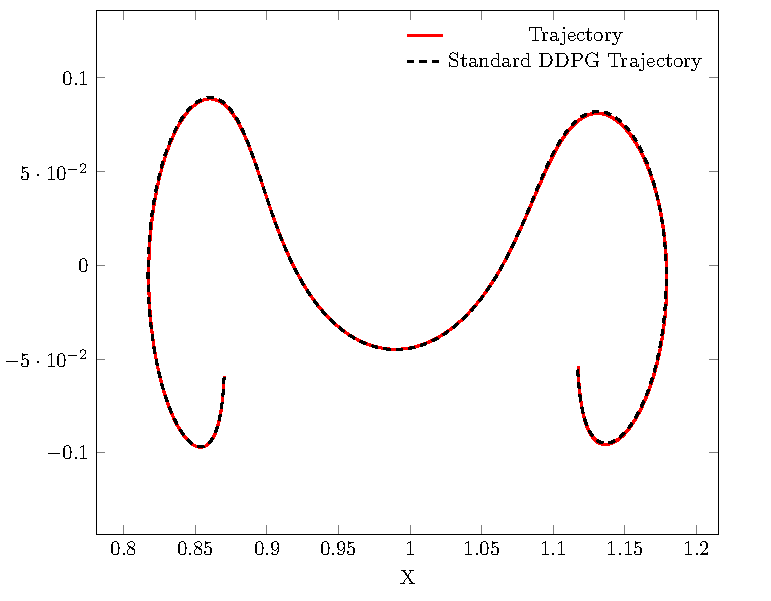
\includegraphics[width=.45\textwidth]{plots/ddpg/trajectory_force/plot_trajectory.pdf}}%
	\subfloat[\lr{MA-DDPG} بازی مجموع‌صفر]{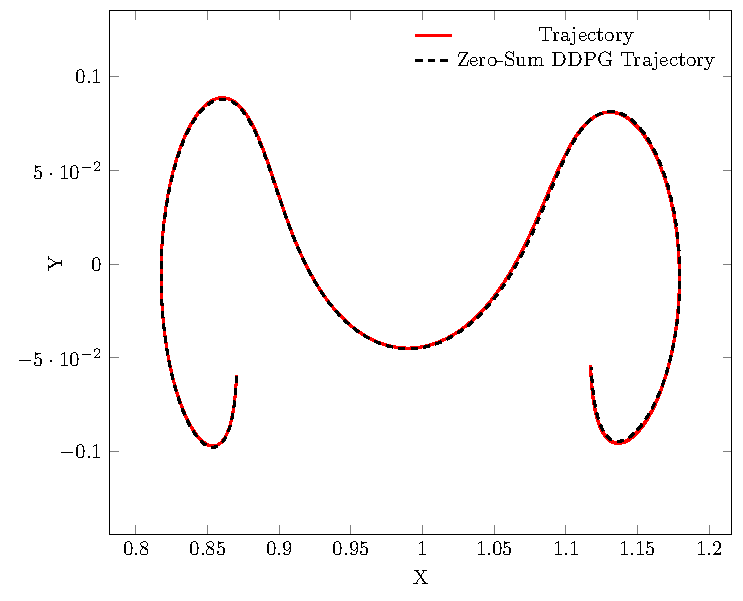
\includegraphics[width=.45\textwidth]{plots/ddpg/trajectory_force/plot_trajectory_zs.pdf}}%
	
	\caption{مسیر طی‌شده فضاپیما با \lr{DDPG} استاندارد و نسخه بازی مجموع‌صفر
		\lr{MA-DDPG}.}
\end{figure}

\subsection{مسیر و فرمان پیشران}
این بخش مسیر و پروفایل فرمان پیشران در طول زمان را برای هر دو نسخه \lr{DDPG} ارائه می‌کند.
\begin{figure}[H]
	\centering
	
	% سطر اول
	\subfloat[\lr{DDPG} استاندارد]{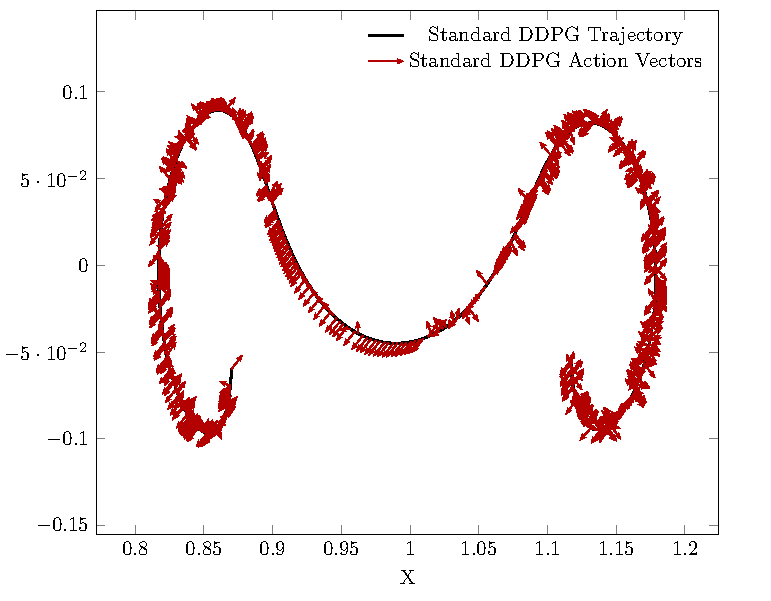
\includegraphics[width=.45\textwidth]{plots/ddpg/trajectory_force/plot_trajectory_force.pdf}}%
	\subfloat[\lr{MA-DDPG} بازی مجموع‌صفر]{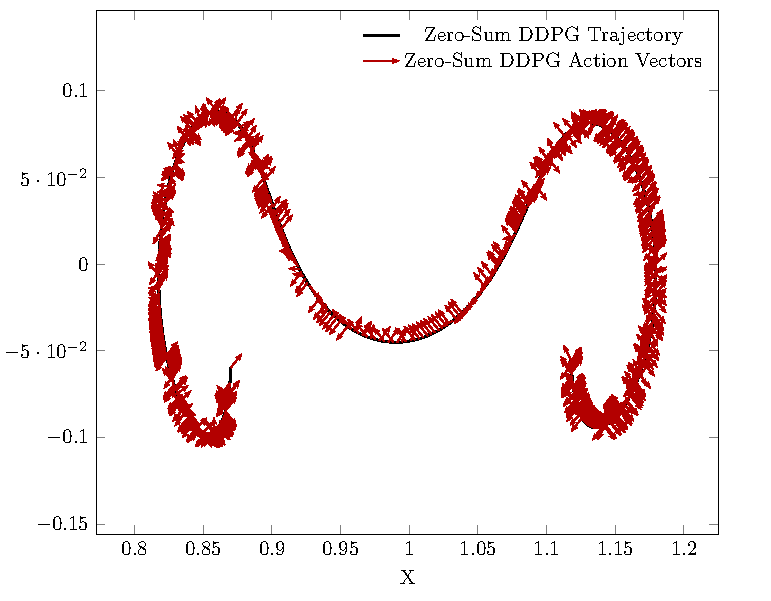
\includegraphics[width=.45\textwidth]{plots/ddpg/trajectory_force/plot_trajectory_force_zs.pdf}}%
	
	\caption{مسیر و فرمان پیشران فضاپیما در \lr{DDPG} استاندارد و نسخه بازی مجموع‌صفر
		\lr{MA-DDPG}.}
\end{figure}


\subsection{توزیع پاداش تجمعی}
این بخش نمودارهای ویولن توزیع پاداش تجمعی را در سناریوهای مختلف برای \lr{DDPG} و \lr{MA-DDPG} نمایش می‌دهد.
\begin{figure}[H]
	\centering
	
	% سطر اول
	\subfloat[شرایط اولیه تصادفی]{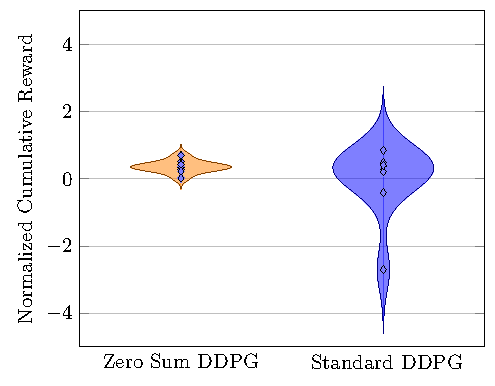
\includegraphics[width=.33\textwidth]{plots/ddpg/violin_plot/initial_condition_shift.pdf}}%
	\subfloat[اغتشاش در عملگرها]{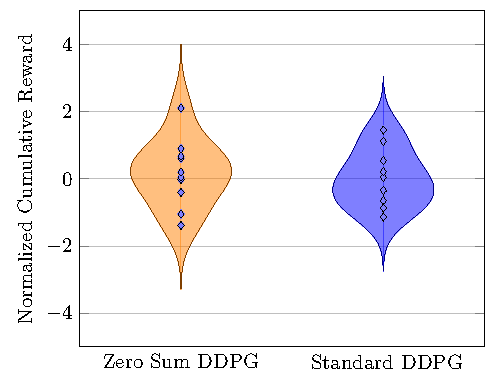
\includegraphics[width=.33\textwidth]{plots/ddpg/violin_plot/actuator_disturbance.pdf}}%
	\subfloat[عدم تطابق مدل]{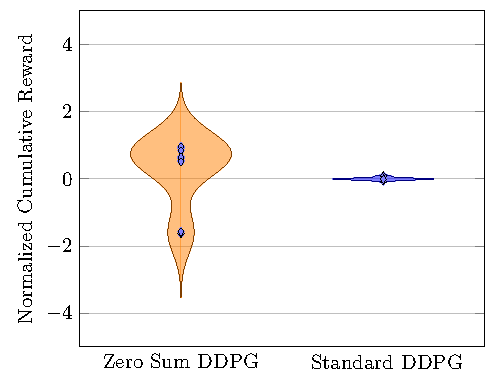
\includegraphics[width=.33\textwidth]{plots/ddpg/violin_plot/model_mismatch.pdf}}\\[1ex]
	
	% سطر دوم
	\subfloat[مشاهده ناقص]{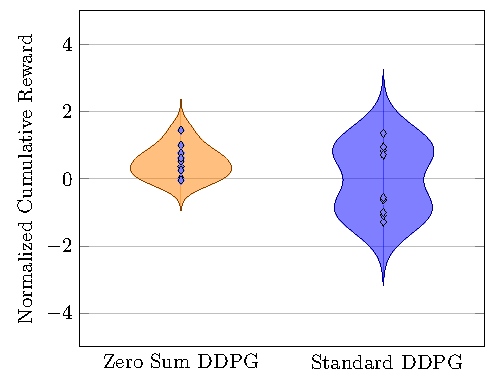
\includegraphics[width=.33\textwidth]{plots/ddpg/violin_plot/partial_observation.pdf}}%
	\subfloat[نویز حسگر]{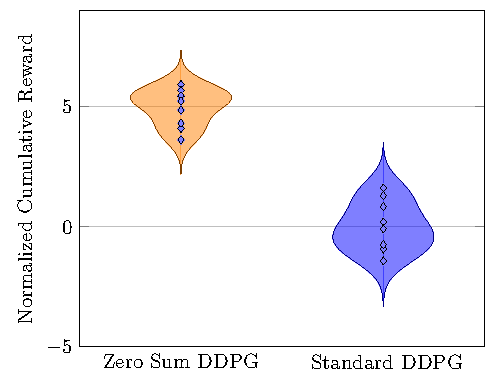
\includegraphics[width=.33\textwidth]{plots/ddpg/violin_plot/sensor_noise.pdf}}%
	\subfloat[تأخیر زمانی]{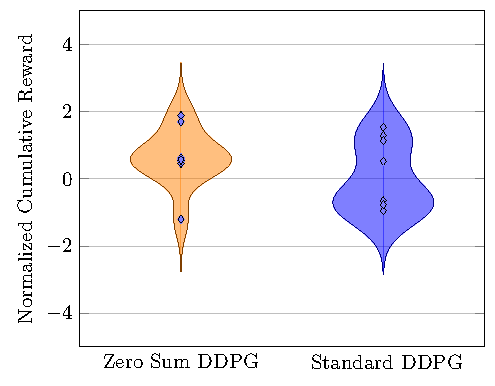
\includegraphics[width=.33\textwidth]{plots/ddpg/violin_plot/time_delay.pdf}}
	
	\caption{مقایسه توزیع پاداش تجمعی در سناریوهای مختلف برای \lr{DDPG} و \lr{MA-DDPG}.}
	\label{fig:ddpg_robustness_violin}
\end{figure}

\subsection{مقایسه عددی}
این بخش شاخص‌های عددی را گزارش می‌کند؛ نتایج بر اساس 100 اجرای مستقل شبیه‌سازی برای هر سناریو به‌دست آمده‌اند.
\begin{table}[H]
	\centering
	\setlength{\tabcolsep}{3pt}
	\small
	\begin{tabular}{@{} R{3.2cm} *{8}{C{1.05cm}} @{}}
		\toprule
		\multirow{2}{*}{\makecell[r]{سناریو}}
		& \multicolumn{2}{c}{پاداش تجمعی} & \multicolumn{2}{c}{مجموع خطای مسیر}
		& \multicolumn{2}{c}{مجموع تلاش کنترلی} & \multicolumn{2}{c}{احتمال شکست} \\
		\cmidrule(lr){2-3}\cmidrule(lr){4-5}\cmidrule(lr){6-7}\cmidrule(lr){8-9}
		& {\rotatebox[origin=c]{90}{\lr{DDPG}}} & {\rotatebox[origin=c]{90}{\lr{MA-DDPG}}}
		& {\rotatebox[origin=c]{90}{\lr{DDPG}}} & {\rotatebox[origin=c]{90}{\lr{MA-DDPG}}}
		& {\rotatebox[origin=c]{90}{\lr{DDPG}}} & {\rotatebox[origin=c]{90}{\lr{MA-DDPG}}}
		& {\rotatebox[origin=c]{90}{\lr{DDPG}}} & {\rotatebox[origin=c]{90}{\lr{MA-DDPG}}} \\
		\midrule
		شرایط اولیه تصادفی
		&
		$-4.17$ & $-3.63$ & $0.40$ & $0.63$ & $5.52$ & $5.60$ & $1.00$ & $1.00$ \\
		اغتشاش در عملگرها
		& $-1.93$ & $-1.96$  & $7.56$ & $7.94$ & $5.60$ & $5.59$ & $0.90$ & $0.30$ \\
		عدم تطابق مدل
		& $-3.24$ & $-2.70$ & $0.70$ & $0.76$ & $5.29$ & $5.57$ & $1.00$ & $1.00$ \\
		مشاهده ناقص
		&
		$-3.28$ & $-2.89$ & $0.68$ & $0.75$ & $5.51$ & $5.57$ & $0.60$ & $0.80$ \\
		نویز حسگر  
		&$-1.07$ & $-0.47$ & $0.10$ & $0.15$ & $5.54$ & $5.54$ & $0.00$ & $0.00$ \\
		تأخیر زمانی        
		&
		$-3.20$ & $-1.91$ & $1.74$ & $2.43$ & $5.61$ & $5.61$ & $0.70$ & $0.70$ \\
		\bottomrule
	\end{tabular}
	\caption{مقایسه عملکرد \lr{DDPG} و \lr{MA-DDPG} در سناریوهای مختلف مقاومت}
	\label{tab:ddpg_comparison}
\end{table}

در جمع‌بندی بر اساس داده‌های جدول، \lr{MA-DDPG} در پنج سناریو پاداش تجمعی بهتری از \lr{DDPG} دارد و تنها در اغتشاش در عملگرها \lr{DDPG} اندکی بهتر است. از نظر مجموع خطای مسیر، \lr{DDPG} در همه سناریوها مقدار کمتری ثبت کرده است. تلاش کنترلی در همه موارد تقریباً برابر است. در احتمال شکست، \lr{MA-DDPG} در اغتشاش در عملگرها بهتر است (0/30 در برابر 0/90)، \lr{DDPG} در مشاهده ناقص بهتر است (0/60 در برابر 0/80) و در سایر سناریوها دو روش برابر هستند.
%\section{الگوریتم \lr{PPO}}
\label{sec:ppo_results}

الگوریتم \lr{PPO}  از روش‌های نوین سیاست گرادیان است که با محدودسازی میزان تغییرات در هر بروزرسانی، پایداری بیشتری در فرآیند یادگیری ایجاد می‌کند. در ادامه، عملکرد این الگوریتم در دو حالت مورد بررسی قرار گرفته است.

\subsection{مسیر طی‌شده}
\begin{figure}[H]
	\centering
	
	% سطر اول
	\subfloat[\lr{PPO} استاندارد]{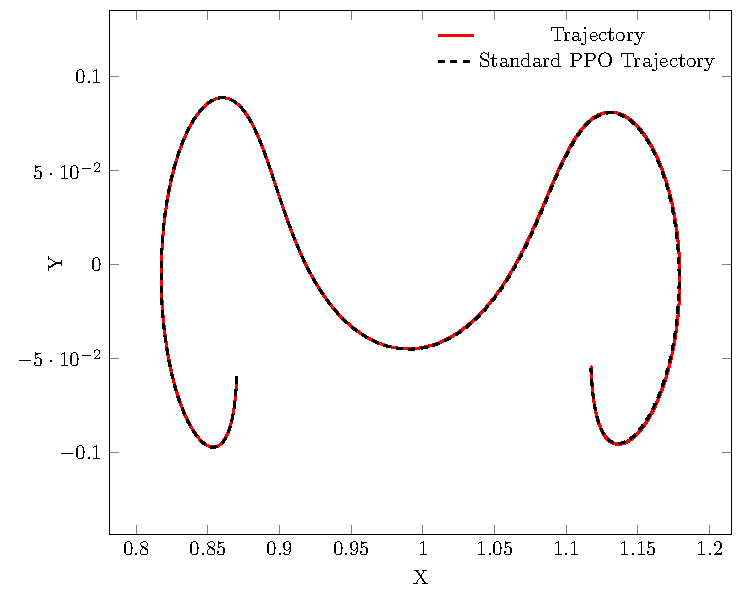
\includegraphics[width=.45\textwidth]{plots/ppo/trajectory_force/plot_trajectory.pdf}}%
	\subfloat[\lr{MA-PPO} بازی مجموع‌صفر]{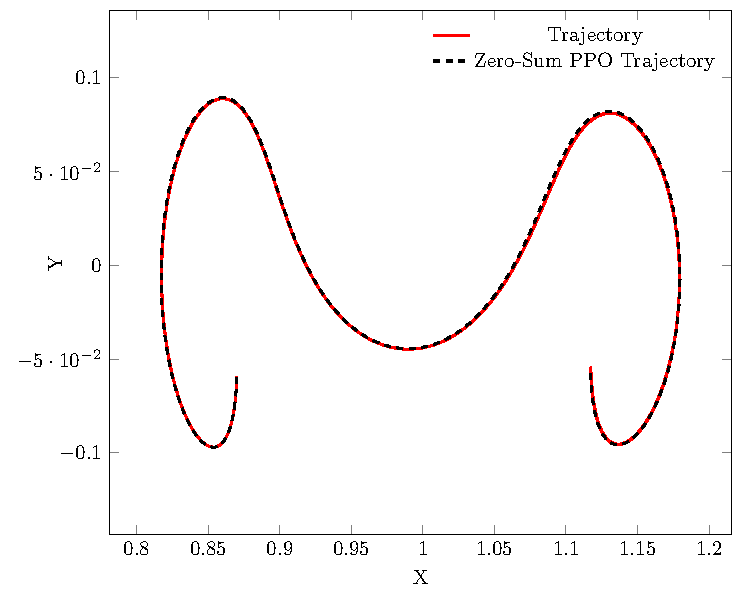
\includegraphics[width=.45\textwidth]{plots/ppo/trajectory_force/plot_trajectory_zs.pdf}}%
	
	\caption{مسیر طی‌شده فضاپیما با \lr{PPO} استاندارد و نسخه بازی مجموع‌صفر \lr{MA-PPO}.}
\end{figure}

\subsection{مسیر و فرمان پیشران}
\begin{figure}[H]
	\centering
	
	% سطر اول
	\subfloat[\lr{PPO} استاندارد]{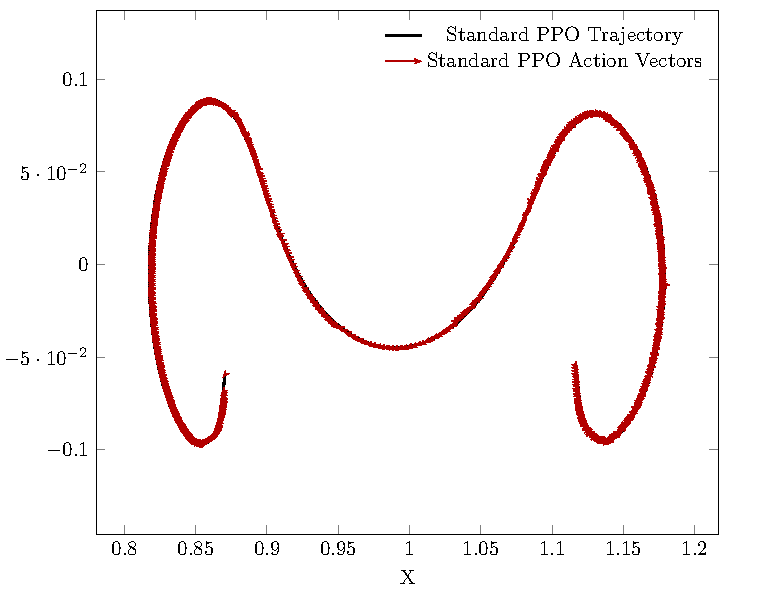
\includegraphics[width=.45\textwidth]{plots/ppo/trajectory_force/plot_trajectory_force.pdf}}%
	\subfloat[\lr{MA-PPO} بازی مجموع‌صفر]{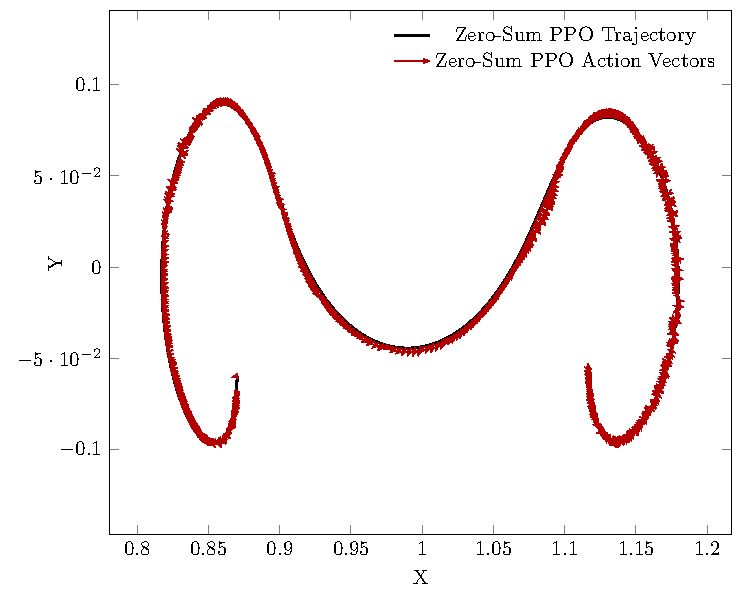
\includegraphics[width=.45\textwidth]{plots/ppo/trajectory_force/plot_trajectory_force_zs.pdf}}%
	
	\caption{مسیر و فرمان پیشران فضاپیما در \lr{PPO} استاندارد و نسخه بازی مجموع‌صفر \lr{MA-PPO}.}
\end{figure}

\subsection{توزیع پاداش تجمعی}
\begin{figure}[H]
	\centering
	
	% سطر اول
	\subfloat[شرایط اولیه تصادفی]{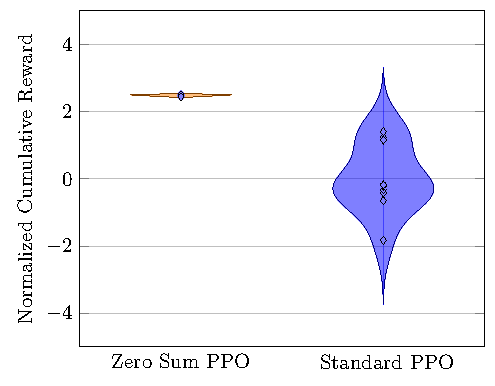
\includegraphics[width=.33\textwidth]{plots/ppo/violin_plot/initial_condition_shift.pdf}}%
	\subfloat[اغتشاش در عملگرها]{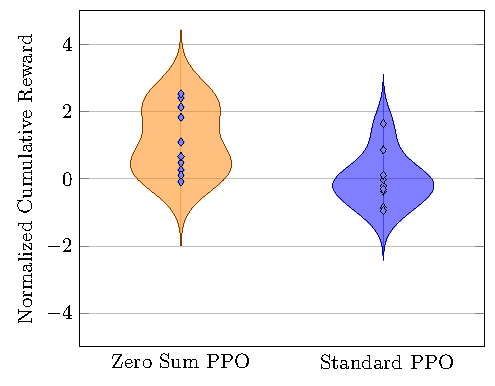
\includegraphics[width=.33\textwidth]{plots/ppo/violin_plot/actuator_disturbance.pdf}}%
	\subfloat[عدم تطابق مدل]{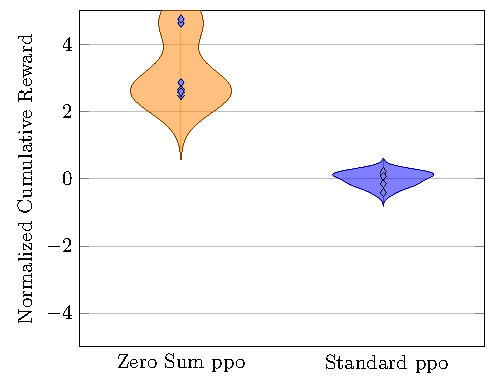
\includegraphics[width=.33\textwidth]{plots/ppo/violin_plot/model_mismatch.pdf}}\\[1ex]
	
	% سطر دوم
	\subfloat[مشاهده ناقص]{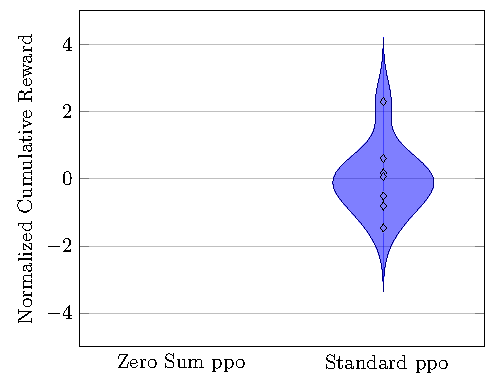
\includegraphics[width=.33\textwidth]{plots/ppo/violin_plot/partial_observation.pdf}}%
	\subfloat[نویز حسگر]{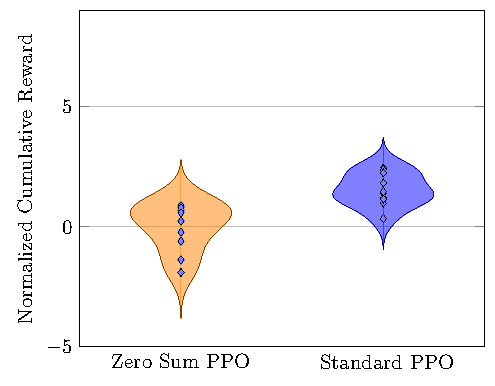
\includegraphics[width=.33\textwidth]{plots/ppo/violin_plot/sensor_noise.pdf}}%
	\subfloat[تأخیر زمانی]{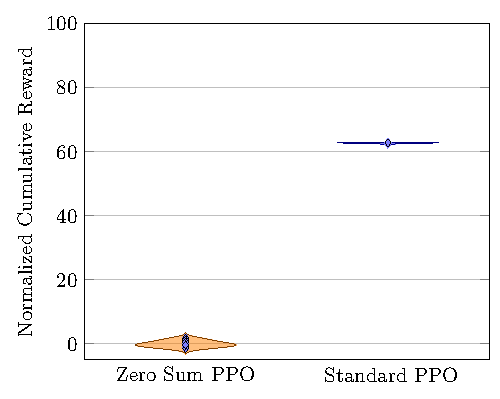
\includegraphics[width=.33\textwidth]{plots/ppo/violin_plot/time_delay.pdf}}
	
	\caption{مقایسه توزیع پاداش تجمعی برای \lr{PPO} و \lr{MA-PPO} در سناریوهای مختلف.}
	\label{fig:ppo_robustness_violin}
\end{figure}

\subsection{مقایسه عددی}
\begin{table}[H]
	\centering
	\setlength{\tabcolsep}{3pt}
	\small
	\begin{tabular}{@{} R{3.2cm} *{8}{C{1.05cm}} @{}}
		\toprule
		\multirow{2}{*}{\makecell[r]{سناریو}}
		& \multicolumn{2}{c}{پاداش تجمعی} & \multicolumn{2}{c}{مجموع خطای مسیر}
		& \multicolumn{2}{c}{مجموع تلاش کنترلی} & \multicolumn{2}{c}{احتمال شکست} \\
		\cmidrule(lr){2-3}\cmidrule(lr){4-5}\cmidrule(lr){6-7}\cmidrule(lr){8-9}
		& {\rotatebox[origin=c]{90}{\lr{PPO}}} & {\rotatebox[origin=c]{90}{\lr{MA-PPO}}}
		& {\rotatebox[origin=c]{90}{\lr{PPO}}} & {\rotatebox[origin=c]{90}{\lr{MA-PPO}}}
		& {\rotatebox[origin=c]{90}{\lr{PPO}}} & {\rotatebox[origin=c]{90}{\lr{MA-PPO}}}
		& {\rotatebox[origin=c]{90}{\lr{PPO}}} & {\rotatebox[origin=c]{90}{\lr{MA-PPO}}} \\
		\midrule
		شرایط اولیه تصادفی
		&
		$-1.85$ & ${0.46}$ & $0.22$ & ${0.14}$ & $1.55$ & $1.98$ & $0.70$ & ${0.00}$ \\
		اغتشاش در عملگرها
		&
		$-1.97$ & ${-1.91}$ & $8.33$ & ${7.50}$ & $2.59$ & $3.42$ & $1.00$ & $1.00$ \\
		عدم تطابق مدل
		&
		${0.46}$ & $0.30$ & ${0.07}$ & $0.08$ & $0.90$ & $1.13$ & $0.00$ & $0.00$ \\
		مشاهده ناقص
		&
		$-3.60$ & ${-1.81}$ & $2.34$ & ${2.06}$ & $1.06$ & $2.15$ & $1.00$ & $1.00$ \\
		نویز حسگر
		&
		${0.52}$ & $0.48$ & ${0.13}$ & $0.15$ & $1.22$ & $2.08$ & $0.00$ & $0.00$ \\
		تأخیر زمانی
		&
		${0.58}$ & $-2.44$ & ${0.03}$ & $2.49$ & $2.43$ & $2.56$ & ${0.00}$ & $1.00$ \\
		\bottomrule
	\end{tabular}
	\caption{مقایسه عملکرد \lr{PPO} و \lr{MA-PPO} در سناریوهای مختلف مقاومت}
	\label{tab:ppo_comparison}
\end{table}

نتایج نشان می‌دهد که الگوریتم \lr{PPO} در حالت بازی مجموع‌صفر عملکرد قابل توجهی دارد، اما تفاوت آن با نسخه استاندارد کمتر از \lr{DDPG} است. این می‌تواند به دلیل ماهیت ذاتی \lr{PPO} در ایجاد تعادل بین اکتشاف و بهره‌برداری باشد که آن را در حالت استاندارد نیز نسبتاً مقاوم می‌سازد.
%\section{الگوریتم \lr{SAC}}
\label{sec:sac_results}

الگوریتم \lr{SAC}  از روش‌های نوین یادگیری تقویتی است که با استفاده از مفهوم آنتروپی، تعادل بهتری بین اکتشاف و بهره‌برداری ایجاد می‌کند. این الگوریتم در شرایط فضاهای پیوسته عملکرد قابل توجهی دارد.

\begin{figure}[H]
	\centering
	
	% سطر اول
	\subfloat[\lr{SAC} استاندارد]{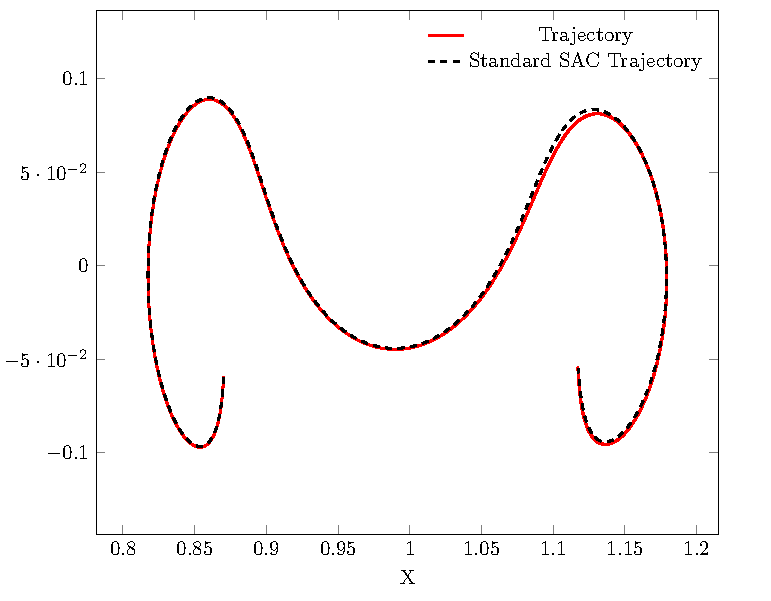
\includegraphics[width=.45\textwidth]{plots/sac/trajectory_force/plot_trajectory.pdf}}%
	\subfloat[\lr{SAC} بازی مجموع‌صفر]{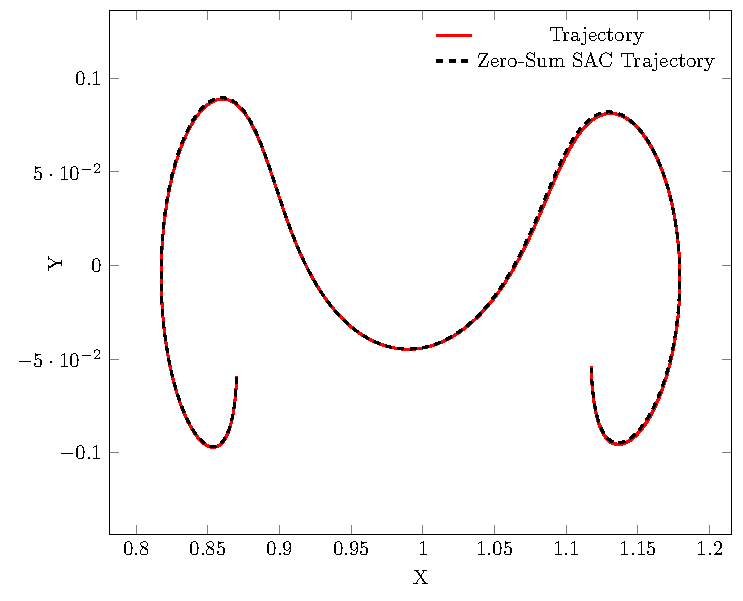
\includegraphics[width=.45\textwidth]{plots/sac/trajectory_force/plot_trajectory_zs.pdf}}%
	
	\caption{مسیر طی‌شده فضاپیما با \lr{SAC} استاندارد و نسخه بازی مجموع‌صفر \lr{MA-SAC}.}
\end{figure}


\begin{figure}[H]
	\centering
	
	% سطر اول
	\subfloat[\lr{SAC} استاندارد]{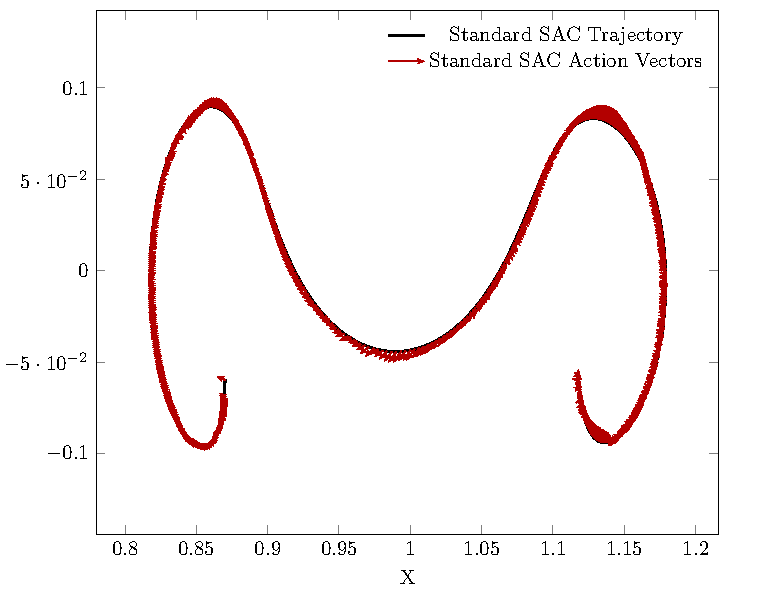
\includegraphics[width=.45\textwidth]{plots/sac/trajectory_force/plot_trajectory_force.pdf}}%
	\subfloat[\lr{SAC} بازی مجموع‌صفر]{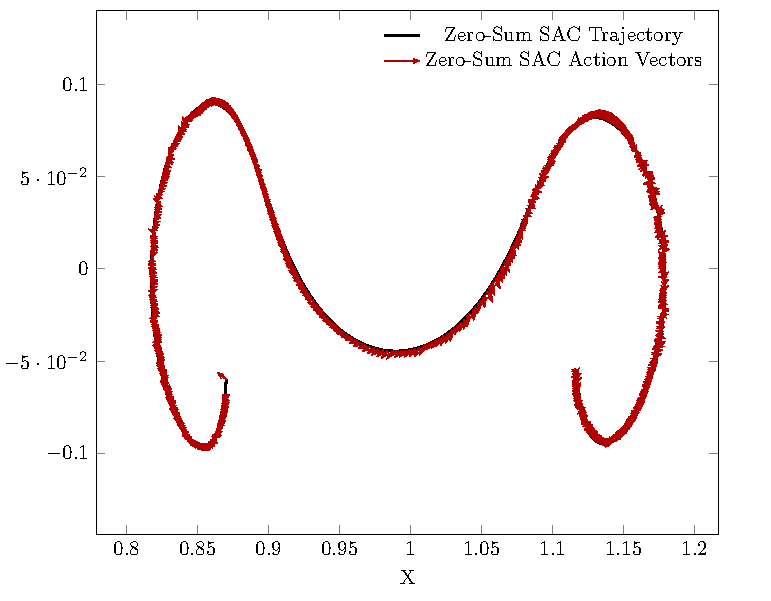
\includegraphics[width=.45\textwidth]{plots/sac/trajectory_force/plot_trajectory_force_zs.pdf}}%
	
	\caption{مسیر و فرمان پیشران فضاپیما در \lr{SAC} استاندارد و نسخه بازی مجموع‌صفر \lr{MA-SAC}.}
\end{figure}

الگوریتم \lr{SAC} در هر دو حالت عملکرد قابل قبولی ارائه می‌دهد. ویژگی خاص این الگوریتم در تنظیم خودکار پارامتر آنتروپی باعث می‌شود که بتواند تعادل مناسبی بین اکتشاف و بهره‌برداری ایجاد کند، اما نسخه بازی مجموع‌صفر آن در شرایط سخت‌تر مقاومت بیشتری نشان می‌دهد.





\begin{table}[H]
	\centering
	\setlength{\tabcolsep}{3pt}
	\small
	\begin{tabular}{@{} R{3.2cm} *{8}{C{1.05cm}} @{}}
		\toprule
		\multirow{2}{*}{\makecell[r]{سناریو}}
		& \multicolumn{2}{c}{پاداش تجمعی} & \multicolumn{2}{c}{مجموع خطای مسیر}
		& \multicolumn{2}{c}{مجموع تلاش کنترلی} & \multicolumn{2}{c}{احتمال شکست} \\
		\cmidrule(lr){2-3}\cmidrule(lr){4-5}\cmidrule(lr){6-7}\cmidrule(lr){8-9}
		& {\rotatebox[origin=c]{90}{\lr{SAC}}} & {\rotatebox[origin=c]{90}{\lr{MA-SAC}}}
		& {\rotatebox[origin=c]{90}{\lr{SAC}}} & {\rotatebox[origin=c]{90}{\lr{MA-SAC}}}
		& {\rotatebox[origin=c]{90}{\lr{SAC}}} & {\rotatebox[origin=c]{90}{\lr{MA-SAC}}}
		& {\rotatebox[origin=c]{90}{\lr{SAC}}} & {\rotatebox[origin=c]{90}{\lr{MA-SAC}}} \\
		\midrule
		شرایط اولیه تصادفی
		&
		$-4.69$ & ${-2.98}$ & $0.29$ & ${0.26}$ & $1.37$ & $1.37$ & $1.00$ & $1.00$ \\
		اغتشاش در عملگرها
		&
		$-1.95$ & ${-1.93}$ & $8.02$ & ${7.72}$ & $3.09$ & $3.09$ & $1.00$ & $1.00$ \\
		عدم تطابق مدل
		&
		$-4.89$ & ${-4.35}$ & $0.38$ & ${0.26}$ & $1.16$ & $1.16$ & $1.00$ & $1.00$ \\
		مشاهده ناقص
		&
		$-3.63$ & ${-0.44}$ & $1.95$ & ${0.07}$ & $1.99$ & $1.99$ & $1.00$ & ${0.00}$ \\
		نویز حسگر
		&
		$-0.89$ & ${0.12}$ & $0.12$ & $0.12$ & $1.86$ & $1.86$ & $0.00$ & $0.00$ \\
		تأخیر زمانی
		&
		$-4.14$ & ${-0.05}$ & $1.87$ & ${0.01}$ & $1.25$ & $1.25$ & $1.00$ & ${0.00}$ \\
		\bottomrule
	\end{tabular}
	\caption{مقایسه عملکرد \lr{SAC} و \lr{MA-SAC} در سناریوهای مختلف مقاومت}
	\label{tab:sac_comparison}
\end{table}
%\section{الگوریتم \lr{TD3}}
\label{sec:td3_results}

الگوریتم \lr{TD3} (یادگیری تفاضل زمانی سه‌گانه عمیق) نسخه بهبودیافته \lr{DDPG} است که با استفاده از تکنیک‌های جدید مانند شبکه‌های دوگانه منتقد و تأخیر در بروزرسانی سیاست، مشکلات تخمین بیش از حد را کاهش می‌دهد.

\subsection{مسیر طی‌شده}
این بخش مسیر طی‌شده فضاپیما را برای نسخه استاندارد و نسخه بازی مجموع‌صفر \lr{TD3} نشان می‌دهد.
\begin{figure}[H]
	\centering
	\subfloat[\lr{TD3} استاندارد]{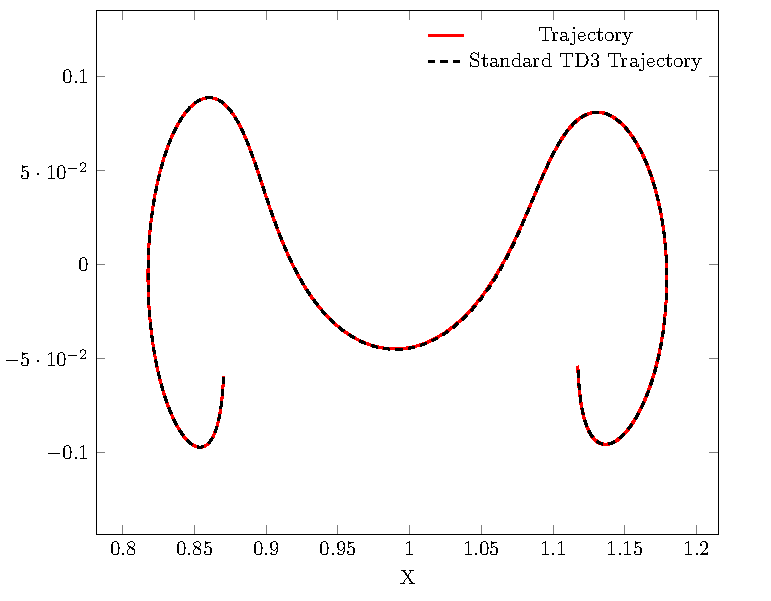
\includegraphics[width=.45\textwidth]{plots/td3/trajectory_force/plot_trajectory.pdf}}%
	\subfloat[\lr{MA-TD3} بازی مجموع‌صفر]{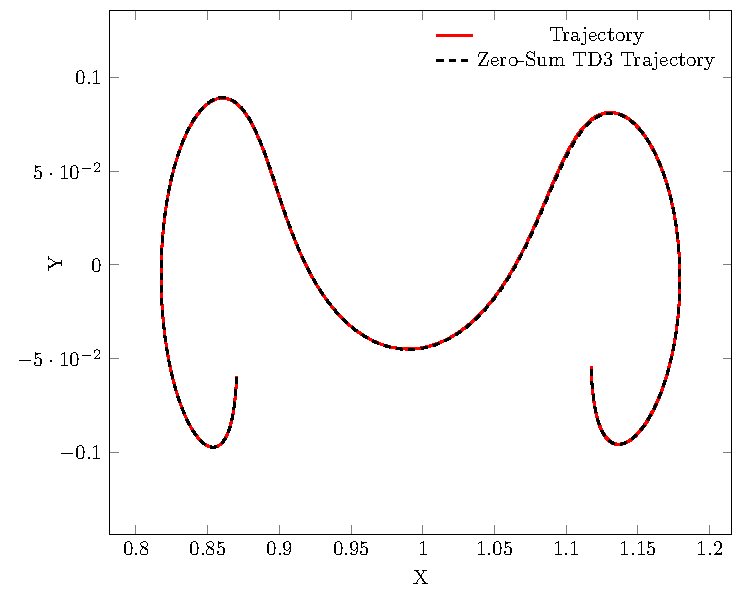
\includegraphics[width=.45\textwidth]{plots/td3/trajectory_force/plot_trajectory_zs.pdf}}%
	\caption{مسیر طی‌شده فضاپیما با \lr{TD3} استاندارد و نسخه بازی مجموع‌صفر \lr{MA-TD3}.}
\end{figure}

\subsection{مسیر و فرمان پیشران}
این بخش مسیر و پروفایل فرمان پیشران در طول زمان را برای هر دو نسخه \lr{TD3} ارائه می‌کند.
\begin{figure}[H]
	\centering
	\subfloat[\lr{TD3} استاندارد]{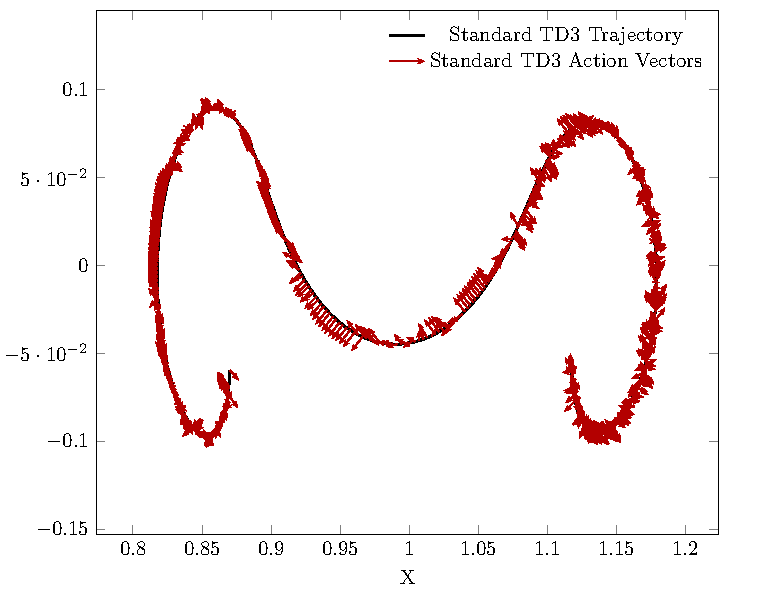
\includegraphics[width=.45\textwidth]{plots/td3/trajectory_force/plot_trajectory_force.pdf}}%
	\subfloat[\lr{MA-TD3} بازی مجموع‌صفر]{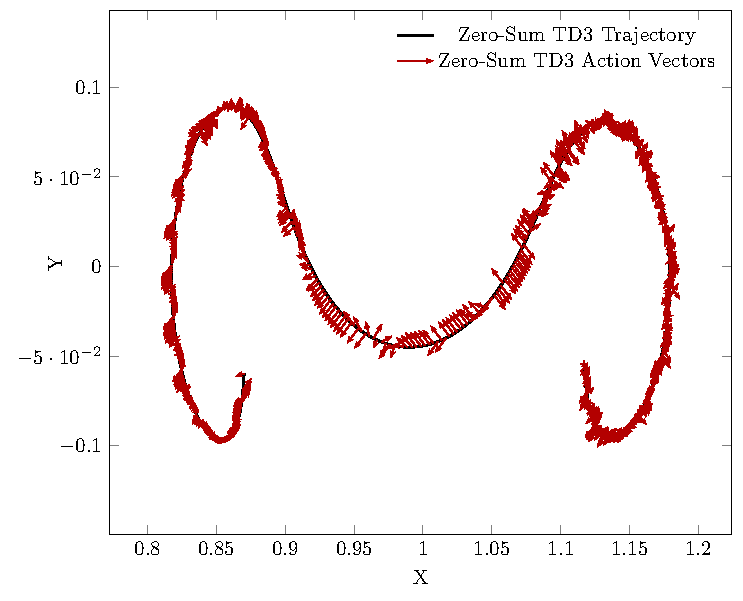
\includegraphics[width=.45\textwidth]{plots/td3/trajectory_force/plot_trajectory_force_zs.pdf}}%
	\caption{مسیر و فرمان پیشران فضاپیما در \lr{TD3} استاندارد و نسخه بازی مجموع‌صفر \lr{MA-TD3}.}
\end{figure}

\subsection{توزیع پاداش تجمعی}
این بخش نمودارهای ویولن توزیع پاداش تجمعی را در سناریوهای مختلف برای \lr{TD3} و \lr{MA-TD3} نمایش می‌دهد.
\begin{figure}[H]
	\centering
	% سطر اول
	\subfloat[شرایط اولیه تصادفی]{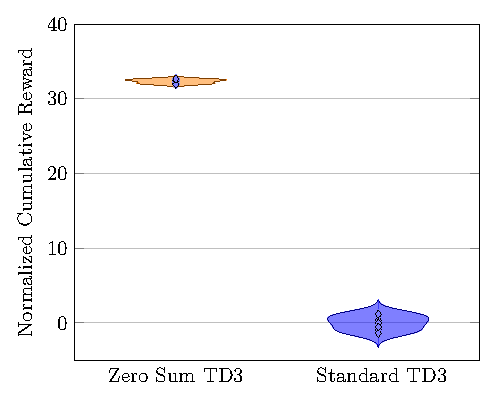
\includegraphics[width=.33\textwidth]{plots/td3/violin_plot/initial_condition_shift.pdf}}%
	\subfloat[اغتشاش در عملگرها]{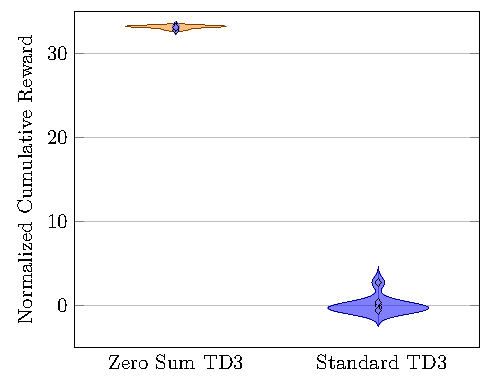
\includegraphics[width=.33\textwidth]{plots/td3/violin_plot/actuator_disturbance.pdf}}%
	\subfloat[عدم تطابق مدل]{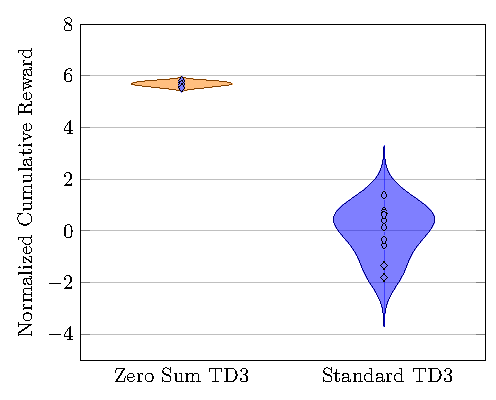
\includegraphics[width=.33\textwidth]{plots/td3/violin_plot/model_mismatch.pdf}}\\[1ex]
	% سطر دوم
	\subfloat[مشاهده ناقص]{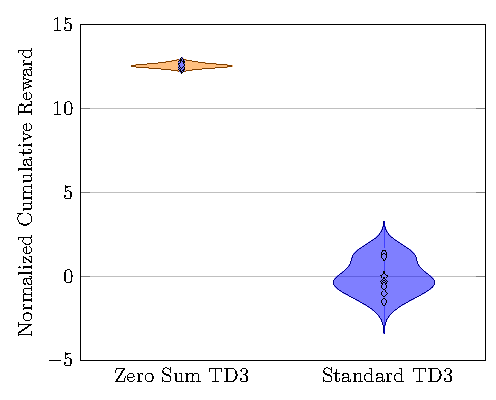
\includegraphics[width=.33\textwidth]{plots/td3/violin_plot/partial_observation.pdf}}%
	\subfloat[نویز حسگر]{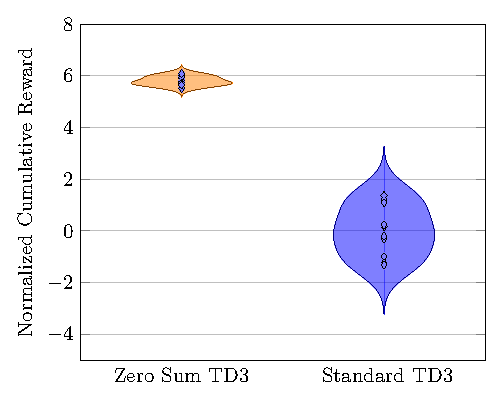
\includegraphics[width=.33\textwidth]{plots/td3/violin_plot/sensor_noise.pdf}}%
	\subfloat[تأخیر زمانی]{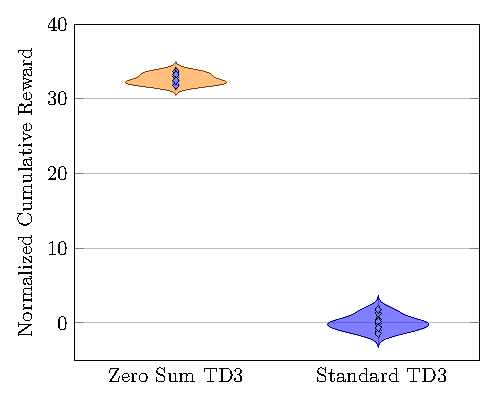
\includegraphics[width=.33\textwidth]{plots/td3/violin_plot/time_delay.pdf}}
	\caption{مقایسه توزیع پاداش تجمعی در سناریوهای مختلف برای \lr{TD3} و \lr{MA-TD3}.}
	\label{fig:td3_robustness_violin}
\end{figure}

\subsection{مقایسه عددی}
این بخش شاخص‌های عددی را گزارش می‌کند؛ نتایج بر اساس 100 اجرای مستقل شبیه‌سازی برای هر سناریو به‌دست آمده‌اند.
\begin{table}[H]
	\centering
	\setlength{\tabcolsep}{3pt}
	\small
	\begin{tabular}{@{} R{3.2cm} *{8}{C{1.05cm}} @{}}
		\toprule
		\multirow{2}{*}{\makecell[r]{سناریو}}
		& \multicolumn{2}{c}{پاداش تجمعی} & \multicolumn{2}{c}{مجموع خطای مسیر}
		& \multicolumn{2}{c}{مجموع تلاش کنترلی} & \multicolumn{2}{c}{احتمال شکست} \\
		\cmidrule(lr){2-3}\cmidrule(lr){4-5}\cmidrule(lr){6-7}\cmidrule(lr){8-9}
		& {\rotatebox[origin=c]{90}{\lr{TD3}}} & {\rotatebox[origin=c]{90}{\lr{MA-TD3}}}
		& {\rotatebox[origin=c]{90}{\lr{TD3}}} & {\rotatebox[origin=c]{90}{\lr{MA-TD3}}}
		& {\rotatebox[origin=c]{90}{\lr{TD3}}} & {\rotatebox[origin=c]{90}{\lr{MA-TD3}}}
		& {\rotatebox[origin=c]{90}{\lr{TD3}}} & {\rotatebox[origin=c]{90}{\lr{MA-TD3}}} \\
		\midrule
		شرایط اولیه تصادفی
		&
		$-2.95$ & ${-0.26}$ & $0.39$ & ${0.14}$ & $5.05$ & $4.57$ & $1.00$ & ${0.30}$\\
		اغتشاش در عملگرها
		&
		$0.56$ & ${0.73}$ & $0.02$ & ${0.00}$ & $3.06$ & $2.66$ & $0.00$ & $0.00$ \\
		عدم تطابق مدل
		&
		$-4.73$ & ${-3.30}$ & $0.47$ & $0.73$ & $5.53$ & $5.41$ & $1.00$ & $1.00$ \\
		مشاهده ناقص
		&
		$0.21$ & ${0.71}$ & $0.02$ & ${0.01}$ & $4.09$ & $3.18$ & $0.00$ & $0.00$ \\
		نویز حسگر
		&
		${-0.08}$ & $-2.93$ & ${0.11}$ & $3.19$ & $5.46$ & $5.50$ & ${0.00}$ & $1.00$ \\
		تأخیر زمانی
		&
		$0.55$ & ${0.67}$ & $0.01$ & $0.01$ & $4.57$ & $4.57$ & $0.00$ & $0.00$ \\
		\bottomrule
	\end{tabular}
	\caption{مقایسه عملکرد \lr{TD3} و \lr{MA-TD3} در سناریوهای مختلف مقاومت}
	\label{tab:td3_comparison}
\end{table}

الگوریتم \lr{TD3} در هر دو حالت عملکرد قابل توجهی دارد، اما نسخه بازی مجموع‌صفر آن بهبودهای معناداری در کیفیت مسیر و مصرف سوخت نشان می‌دهد. ثبات بیشتر این الگوریتم در مقایسه با \lr{DDPG} در هر دو نسخه قابل مشاهده است.
%\section{نتایج نسخه استاندارد}
\label{sec:std_results}
در این بخش، نتایج نسخه‌های تک‌عاملی الگوریتم‌ها در سناریوهای مقاومت مختلف ارائه و تحلیل می‌شود.

\subsection{توزیع پاداش تجمعی}
\begin{figure}[H]
	\centering
	
	% سطر اول
	\subfloat[شرایط اولیه تصادفی]{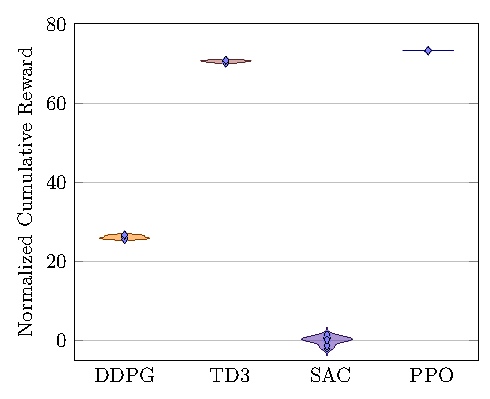
\includegraphics[width=.33\textwidth]{plots/standard/violin_plot/initial_condition_shift.pdf}}%
	\subfloat[اغتشاش در عملگرها]{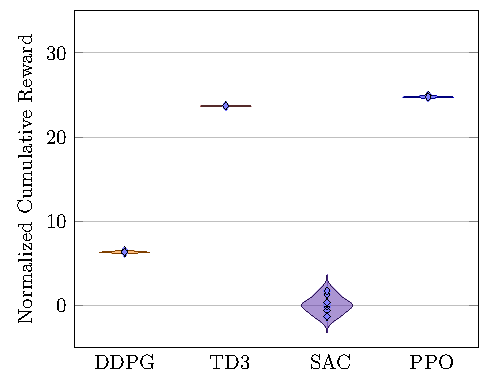
\includegraphics[width=.33\textwidth]{plots/standard/violin_plot/actuator_disturbance.pdf}}%
	\subfloat[عدم تطابق مدل]{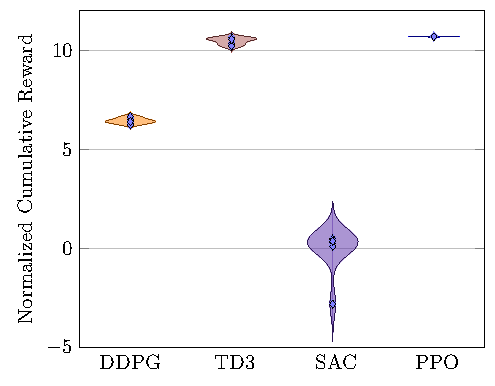
\includegraphics[width=.33\textwidth]{plots/standard/violin_plot/model_mismatch.pdf}}\\[1ex]
	
	% سطر دوم
	\subfloat[مشاهده ناقص]{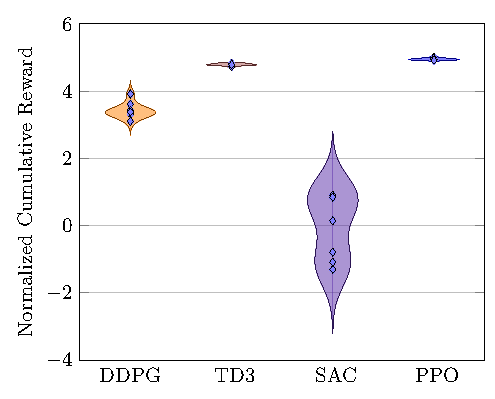
\includegraphics[width=.33\textwidth]{plots/standard/violin_plot/partial_observation.pdf}}%
	\subfloat[نویز حسگر]{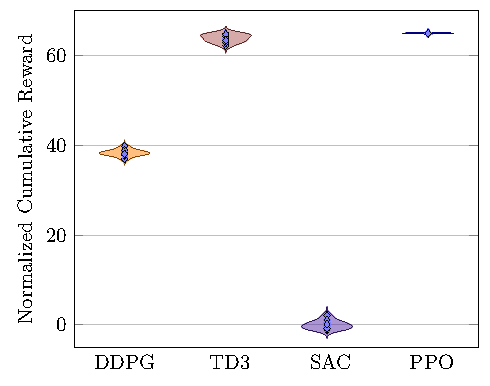
\includegraphics[width=.33\textwidth]{plots/standard/violin_plot/sensor_noise.pdf}}%
	\subfloat[تأخیر زمانی]{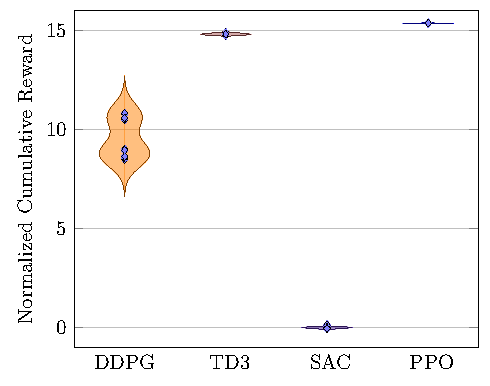
\includegraphics[width=.33\textwidth]{plots/standard/violin_plot/time_delay.pdf}}
	
	\caption{مقایسه توزیع پاداش تجمعی برای نسخه‌های تک‌عاملی  در سناریوهای مختلف.}
	\label{fig:std_robustness_violin}
\end{figure}

\subsection{مقایسه عددی}
\begin{table}[H]
	\centering
	\setlength{\tabcolsep}{6pt}
	\renewcommand{\arraystretch}{1.5}
	\scriptsize
	
	% --- Row 1: left + right boxes, centered as a group ---
	\makebox[\linewidth][c]{%
		\parbox{.48\linewidth}{
			\centering
			\footnotesize
			\begin{tabular}{@{} R {2.6cm}*{4}{c}}
				\toprule
				{سناریو} & \lr{DDPG} & \lr{PPO} & \lr{SAC} & \lr{TD3} \\
				\midrule
				شرایط اولیه تصادفی & $-0.27$ & $0.61$ & $-0.76$ & $0.56$ \\
				اغتشاش در عملگرها & $-0.38$ & $0.61$ & $-0.72$ & $0.55$ \\
				عدم تطابق مدل      & $-0.84$ & $0.58$ & $-2.98$ & $0.51$ \\
				مشاهده ناقص        & $-0.88$ & $0.36$ & $-3.65$ & $0.23$ \\
				نویز حسگر          & $-0.85$ & $0.58$ & $-2.90$ & $0.52$ \\
				تأخیر زمانی        & $-0.76$ & $0.61$ & $-2.98$ & $0.48$ \\
				\bottomrule
			\end{tabular}
			\caption*{\normalfont پاداش تجمعی}
		}
		\hspace{0.04\linewidth}
		\parbox{.48\linewidth}{
			\centering
			\footnotesize
			\begin{tabular}{@{} R {2.6cm}*{4}{c}}
				\toprule
				{سناریو} & \lr{DDPG} & \lr{PPO} & \lr{SAC} & \lr{TD3} \\
				\midrule
				شرایط اولیه تصادفی & $3.30$ & $2.56$ & $8.06$ & $0.72$ \\
				اغتشاش در عملگرها & $3.74$ & $2.58$ & $7.91$ & $0.77$ \\
				عدم تطابق مدل      & $10.87$ & $3.06$ & $17.12$ & $1.09$ \\
				مشاهده ناقص        & $8.18$ & $3.34$ & $15.47$ & $1.77$ \\
				نویز حسگر          & $11.04$ & $3.08$ & $16.81$ & $1.02$ \\
				تأخیر زمانی        & $8.95$ & $2.27$ & $15.70$ & $0.81$ \\
				\bottomrule
			\end{tabular}
			\caption*{\normalfont مجموع خطای مسیر}
		}%
	}
	
	\vspace{0.6em}
	
	% --- Row 2: left + right boxes, centered as a group ---
	\makebox[\linewidth][c]{%
		\parbox{.48\linewidth}{
			\centering
			\footnotesize
			\begin{tabular}{@{} R {2.6cm}*{4}{c}}
				\toprule
				{سناریو} & \lr{DDPG} & \lr{PPO} & \lr{SAC} & \lr{TD3} \\
				\midrule
				شرایط اولیه تصادفی & $5.11$ & $0.77$ & $1.76$ & $3.31$ \\
				اغتشاش در عملگرها & $4.89$ & $0.77$ & $1.71$ & $3.07$ \\
				عدم تطابق مدل      & $5.48$ & $0.86$ & $2.37$ & $4.32$ \\
				مشاهده ناقص        & $5.37$ & $1.03$ & $2.33$ & $4.10$ \\
				نویز حسگر          & $5.48$ & $0.86$ & $2.37$ & $4.30$ \\
				تأخیر زمانی        & $5.51$ & $0.76$ & $2.11$ & $5.12$ \\
				\bottomrule
			\end{tabular}
			\caption*{\normalfont مجموع تلاش کنترلی}
		}
		\hspace{0.04\linewidth}
		\parbox{.48\linewidth}{
			\centering
			\footnotesize
			\begin{tabular}{@{} R {2.6cm}*{4}{c}}
				\toprule
				{سناریو} & \lr{DDPG} & \lr{PPO} & \lr{SAC} & \lr{TD3} \\
				\midrule
				شرایط اولیه تصادفی & $0.00$ & $0.00$ & $0.00$ & $0.00$ \\
				اغتشاش در عملگرها & $0.00$ & $0.00$ & $0.00$ & $0.00$ \\
				عدم تطابق مدل      & $0.00$ & $0.00$ & $1.00$ & $0.00$ \\
				مشاهده ناقص        & $0.00$ & $0.00$ & $1.00$ & $0.00$ \\
				نویز حسگر          & $0.00$ & $0.00$ & $1.00$ & $0.00$ \\
				تأخیر زمانی        & $0.00$ & $0.00$ & $1.00$ & $0.00$ \\
				\bottomrule
			\end{tabular}
			\caption*{\normalfont احتمال شکست}
		}%
	}
	
	\caption{مقایسه الگوریتم‌های چندعاملی در سناریوهای مختلف مقاومت}
\end{table}


%\subsection{تحلیل و بحث}
بر اساس داده‌ها، \lr{TD3} به‌طور پایدار بالاترین پاداش و کمترین خطای مسیر را ثبت می‌کند، درحالی‌که \lr{PPO} کمترین تلاش کنترلی را دارد. \lr{SAC} در برخی سناریوهای دشوار (عدم تطابق مدل، مشاهده ناقص، نویز حسگر، تأخیر زمانی) نرخ شکست بالاتری نشان می‌دهد و \lr{DDPG} عموماً از نظر پاداش و خطا ضعیف‌تر از \lr{PPO} و \lr{TD3} است.

 
%\section{نتایج نسخه چندعاملی}
\label{sec:zs_results}
در این بخش، عملکرد الگوریتم‌ها در حالت چندعاملیِ بازی مجموع‌صفر ارائه و تحلیل می‌شود.

\subsection{توزیع پاداش تجمعی}
\begin{figure}[H]
	\centering
	
	% سطر اول
	\subfloat[شرایط اولیه تصادفی]{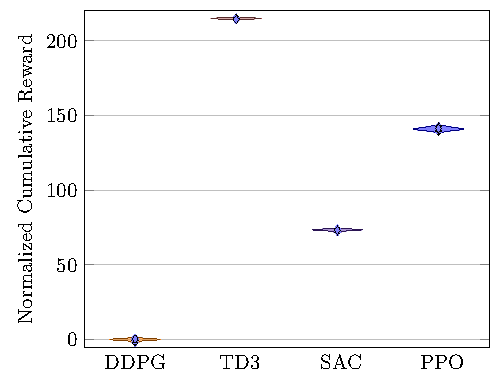
\includegraphics[width=.33\textwidth]{plots/ZeroSum/violin_plot/initial_condition_shift.pdf}}%
	\subfloat[اغتشاش در عملگرها]{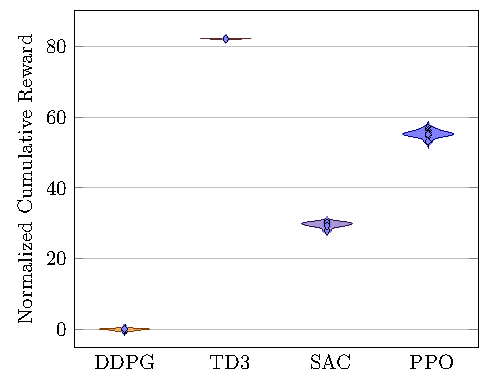
\includegraphics[width=.33\textwidth]{plots/ZeroSum/violin_plot/actuator_disturbance.pdf}}%
	\subfloat[عدم تطابق مدل]{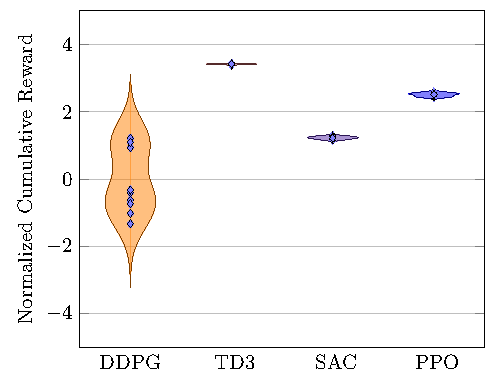
\includegraphics[width=.33\textwidth]{plots/ZeroSum/violin_plot/model_mismatch.pdf}}\\[1ex]
	
	% سطر دوم
	\subfloat[مشاهده ناقص]{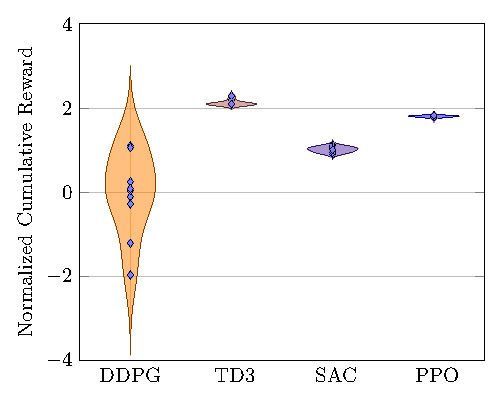
\includegraphics[width=.33\textwidth]{plots/ZeroSum/violin_plot/partial_observation.pdf}}%
	\subfloat[نویز حسگر]{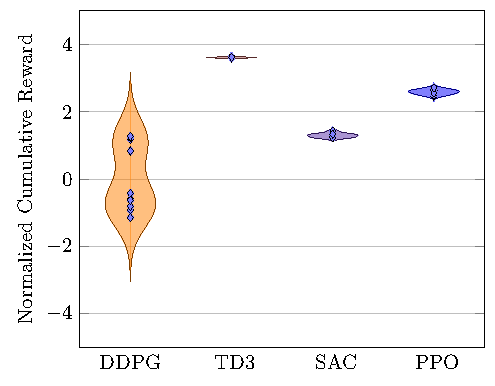
\includegraphics[width=.33\textwidth]{plots/ZeroSum/violin_plot/sensor_noise.pdf}}%
	\subfloat[تأخیر زمانی]{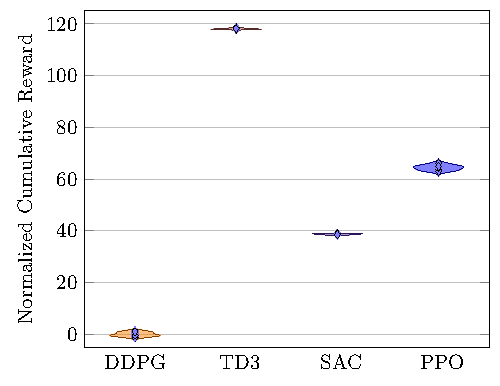
\includegraphics[width=.33\textwidth]{plots/ZeroSum/violin_plot/time_delay.pdf}}
	
	\caption{مقایسه توزیع پاداش تجمعی برای الگوریتم‌ها در حالت چندعاملی  در سناریوهای مختلف.}
	\label{fig:zs_robustness_violin}
\end{figure}

\subsection{مقایسه عددی}
\begin{table}[H]
	\centering
	\setlength{\tabcolsep}{6pt}      % tighter columns (built-in)
	\renewcommand{\arraystretch}{1.5}% a bit more row height (built-in)
	\scriptsize                      % smaller font to fit
	
	% --- Row 1: left + right boxes, centered as a group ---
	\makebox[\linewidth][c]{%
		\parbox{.48\linewidth}{
			\centering
			\footnotesize
			\begin{tabular}{@{} R {2.6cm}*{4}{c}}
				\toprule
				{سناریو} & \lr{DDPG} & \lr{PPO} & \lr{SAC} & \lr{TD3} \\
				\midrule
				شرایط اولیه تصادفی & $-0.41$ & $0.34$ & $-0.02$ & ${0.74}$ \\
				اغتشاش در عملگرها & $-0.44$ & $0.35$ & $-0.02$ & ${0.73}$ \\
				عدم تطابق مدل      & $-0.63$ & $0.38$ & $-0.13$ & ${0.75}$ \\
				مشاهده ناقص        & $-1.52$ & $0.40$ & $-0.44$ & ${0.71}$ \\
				نویز حسگر          & $-0.60$ & $0.37$ & $-0.12$ & ${0.75}$ \\
				تأخیر زمانی        & $-1.19$ & $0.17$ & $-0.05$ & ${0.67}$ \\
				\bottomrule
			\end{tabular}
			\caption*{\normalfont پاداش تجمعی}
		}
		\hspace{0.04\linewidth}
		\parbox{.48\linewidth}{
			\centering
			\footnotesize
			\begin{tabular}{@{} R {2.6cm}*{4}{c}}
				\toprule
				{سناریو} & \lr{DDPG} & \lr{PPO} & \lr{SAC} & \lr{TD3} \\
				\midrule
				شرایط اولیه تصادفی & $4.42$ & $4.30$ & $4.02$ & ${1.22}$ \\
				اغتشاش در عملگرها & $4.39$ & $4.38$ & $4.01$ & ${1.26}$ \\
				عدم تطابق مدل      & $8.85$ & $3.57$ & $4.78$ & ${1.25}$ \\
				مشاهده ناقص        & $9.65$ & $2.44$ & $5.17$ & ${1.09}$ \\
				نویز حسگر          & $9.12$ & $3.58$ & $4.66$ & ${1.25}$ \\
				تأخیر زمانی        & $6.73$ & $4.53$ & $4.12$ & ${1.21}$ \\
				\bottomrule
			\end{tabular}
			\caption*{\normalfont مجموع خطای مسیر}
		}%
	}
	
	\vspace{0.6em}
	
	% --- Row 2: left + right boxes, centered as a group ---
	\makebox[\linewidth][c]{%
		\parbox{.48\linewidth}{
			\centering
			\footnotesize
			\begin{tabular}{@{} R {2.6cm}*{4}{c}}
				\toprule
				{سناریو} & \lr{DDPG} & \lr{PPO} & \lr{SAC} & \lr{TD3} \\
				\midrule
				شرایط اولیه تصادفی & $5.40$ & $1.15$ & $1.34$ & $2.76$ \\
				اغتشاش در عملگرها & $5.08$ & $1.11$ & $1.23$ & $2.66$ \\
				عدم تطابق مدل      & $5.55$ & $1.51$ & $2.09$ & $3.38$ \\
				مشاهده ناقص        & $5.46$ & $1.50$ & $2.00$ & $3.20$ \\
				نویز حسگر          &$5.54$ & $1.52$ & $2.08$ & $3.38$ \\
				تأخیر زمانی        & $5.48$ & $1.25$ & $1.25$ & $4.57$ \\
				\bottomrule
			\end{tabular}
			\caption*{\normalfont مجموع تلاش کنترلی}
		}
		\hspace{0.04\linewidth}
		\parbox{.48\linewidth}{
			\centering
			\footnotesize
			\begin{tabular}{@{} R {2.6cm}*{4}{c}}
				\toprule
				{سناریو} & \lr{DDPG} & \lr{PPO} & \lr{SAC} & \lr{TD3} \\
				\midrule
				شرایط اولیه تصادفی & $0.00$ & $0.00$ & $0.00$ & $0.00$ \\
				اغتشاش در عملگرها & $0.00$ & $0.00$ & $0.00$ & $0.00$ \\
				عدم تطابق مدل      & $0.00$ & $0.00$ & $0.20$ & $0.00$ \\
				مشاهده ناقص        & $0.00$ & $0.00$ & $0.20$ & $0.00$ \\
				نویز حسگر          & $0.00$ & $0.00$ & $0.20$ & $0.00$ \\
				تأخیر زمانی        & $0.00$ & $0.00$ & $0.20$ & $0.00$ \\
				\bottomrule
			\end{tabular}
			\caption*{\normalfont احتمال شکست}
		}%
	}
	
	\caption{مقایسه الگوریتم‌های چندعاملی در سناریوهای مختلف مقاومت}
\end{table}

%\subsection{تحلیل و بحث}
در حالت چندعاملی، \lr{TD3}
  به‌طور پایدار پاداش بالاتر و خطای مسیر کمتر ثبت می‌کند، در حالی‌که \lr{PPO} کمترین تلاش کنترلی را نشان می‌دهد. عملکرد \lr{SAC} و \lr{DDPG} در برخی سناریوهای دشوار ضعیف‌تر است، هرچند نرخ‌های شکست عمدتاً پایین باقی می‌ماند. 





























